\documentclass[11pt,a4paper]{article}

\usepackage[utf8]{inputenc}
\usepackage[T1]{fontenc}
\usepackage[spanish]{babel}
\usepackage{lmodern}
\usepackage[a4paper,margin=2.5cm]{geometry}
\usepackage{graphicx}
\usepackage{booktabs}
\usepackage{caption}
\usepackage{microtype}
\usepackage{parskip}
\usepackage{xcolor}
\usepackage[colorlinks=true,linkcolor=black,urlcolor=blue,citecolor=black]{hyperref}
\usepackage{titling}
\usepackage{titlesec}

% Espaciado de secciones más cómodo
\titlespacing*{\section}{0pt}{18pt}{8pt}
\titlespacing*{\subsection}{0pt}{14pt}{6pt}

% Sin numeración profunda; solo sección
\setcounter{secnumdepth}{1}

\setlength{\droptitle}{-2cm}

\title{\textbf{Segmentación de clientes en una plataforma de comercio electrónico}\\
\large Análisis no supervisado sobre datos de Google Analytics}
\author{Andrés Fernando Gómez Rojas}
\date{\today}

\begin{document}

\maketitle

\begin{abstract}
\noindent
Se aborda el problema de segmentar visitantes de un sitio de comercio electrónico
a partir de datos de comportamiento de Google Analytics, con el objetivo de
proveer al equipo de marketing grupos accionables para personalizar campañas y
optimizar inversión. A partir de un dataset de 9.996 visitantes únicos
pre-agregados, se aplica un pipeline que parte de un análisis exploratorio
riguroso, atraviesa una etapa de feature engineering justificada en hallazgos
concretos del exploratorio, compara seis algoritmos de clustering y termina con
una validación estadística formal de los segmentos obtenidos. La solución final
emplea KMeans con cuatro clusters, elegida por el balance entre métricas
internas, estabilidad bajo bootstrap y accionabilidad de los segmentos para
marketing. Los cuatro grupos identificados (Desktop Engaged, Desktop Frecuente,
Weekend Warriors y Mobile Users) muestran diferencias estadísticamente
significativas y, lo que es más relevante, con effect size grande. El análisis
revela además que el dispositivo es el separador dominante por encima del canal
de adquisición, contradiciendo un supuesto habitual en marketing digital.
\end{abstract}

\section{Introducción}

Para una empresa de comercio electrónico, entender a sus visitantes en grupos
diferenciados es un insumo directo para la toma de decisiones de marketing.
Permite personalizar campañas, distribuir presupuesto entre canales con criterio
y diseñar experiencias adaptadas al tipo de usuario. Este informe documenta el
ejercicio de segmentar los visitantes de un sitio web a partir de información de
comportamiento extraída de Google Analytics, sin variables de conversión ni de
revenue, por lo que el objetivo es descriptivo y operativo más que predictivo.

El dataset entregado contiene 9.996 filas y trece variables que mezclan
identificadores, métricas de actividad y atributos de dispositivo y canal. Una
observación temprana define todo el enfoque del trabajo: cada fila corresponde a
un visitante único, no a una sesión. La columna llamada \texttt{sessionId} no
es un identificador sino el número de sesiones que realizó cada visitante, con
rango entre uno y doscientas setenta y ocho. Las variables \texttt{weekend\_prop},
\texttt{bounce\_prop} y \texttt{device.isMobile} son proporciones agregadas a
través de las sesiones del visitante. Reconocer esto temprano evita malinterpretar
los datos y permite abordar el problema directamente como una segmentación a
nivel persona, sin necesidad de agregar antes.

\section{Análisis exploratorio}

El análisis exploratorio cumple en este trabajo dos propósitos. Por una parte,
verificar la calidad de los datos y caracterizar las variables. Por otra,
producir hallazgos que justifiquen las decisiones de preprocesamiento que vienen
después. Toda transformación posterior debe rastrearse a una observación concreta
del exploratorio.

La calidad del dataset es notablemente buena. No hay valores nulos en ninguna de
las columnas, no hay duplicados completos, y todas las restricciones lógicas se
cumplen: las proporciones están entre cero y uno, las horas entre cero y
veintitrés, los pageviews nunca exceden los hits, y cada visitante aparece una
sola vez. Solo cuatro visitantes presentan valores intermedios en
\texttt{device.isMobile}, lo que indica que cambiaron de dispositivo entre
sesiones. La composición del dataset sugiere fuertemente que se trata de la
muestra de Google Merchandise Store usada históricamente para tutoriales de
Google Analytics: noventa por ciento de visitantes en desktop, ochenta y nueve
por ciento usando Chrome, cincuenta y seis por ciento en Macintosh. Reconocer
este sesgo del origen es relevante para interpretar después la representatividad
de los segmentos mobile.

Las distribuciones de las variables de conteo son extremadamente sesgadas a la
derecha. La skewness de \texttt{n\_sessions} supera los diecinueve y su kurtosis
se acerca a seiscientos sesenta, lo que confirma una cola pesadísima dominada
por unos pocos visitantes con cientos de sesiones. Las variables \texttt{totals.hits}
y \texttt{totals.pageviews} presentan también skewness por encima de cinco. Esto
tiene dos implicaciones técnicas. Primero, ninguna prueba paramétrica que asuma
normalidad será apropiada para estas variables, por lo que descartamos ANOVA en
favor de Kruskal-Wallis, y Pearson en favor de Spearman. Segundo, antes de
aplicar cualquier algoritmo basado en distancia euclidiana es necesario
transformar estas variables para que un puñado de outliers no dominen las
distancias.

El análisis bivariado revela dos redundancias importantes. La primera, entre
\texttt{totals.hits} y \texttt{totals.pageviews}, con correlación de Spearman de
0.97 y factor de inflación de varianza por encima de veintisiete. La segunda,
entre \texttt{channelGrouping} y \texttt{trafficSource.medium}, con un V de
Cramer de 0.98, prácticamente la misma variable expresada en dos formas. Estas
redundancias se atienden en el preprocesamiento eliminando una de las dos
variables del segundo par y derivando una métrica complementaria del primero.

Un hallazgo del exploratorio que merece destacarse, porque anticipa la
estructura del clustering posterior, es la correlación negativa de Spearman
entre \texttt{n\_sessions} y \texttt{totals.hits}, con valor de -0.64. Quien
viene más veces tiene menos hits totales que quien viene pocas veces. La
interpretación que damos es que coexisten dos comportamientos opuestos en la
base de visitantes: personas que vienen una o dos veces y realizan sesiones
extensas de investigación, y personas que vienen muchas veces pero hacen
sesiones cortas de chequeo rápido. Esta dualidad se va a recuperar después como
dos clusters distintos.

Para cerrar el exploratorio se aplicó Isolation Forest sobre las variables
numéricas con un nivel de contaminación del cinco por ciento, lo que identifica
visitantes con combinaciones inusuales de comportamiento que no necesariamente
son outliers en una variable aislada. Los outliers multivariados resultan ser
visitantes con engagement aproximadamente cinco veces superior al típico, y el
separador más fuerte entre outliers y resto es \texttt{weekend\_prop}. Esto
anticipa, antes siquiera de hacer clustering, la existencia de un segmento de
visitantes muy activos en fin de semana. La decisión sobre estos outliers es no
eliminarlos: son precisamente los power users que el negocio querría identificar.
En cambio, se tratan con clip al percentil 99 y transformación logarítmica antes
del clustering.

\section{Preprocesamiento}

Todas las decisiones de preprocesamiento se derivan de observaciones del
análisis exploratorio. No hay transformaciones aplicadas por inercia.

Las variables de conteo \texttt{n\_sessions}, \texttt{totals.hits} y
\texttt{totals.pageviews}, junto con sus derivadas \texttt{hits\_per\_session} y
\texttt{pageviews\_per\_session}, se truncan al percentil 99 y luego se aplica
\texttt{log1p}. El clip evita que cinco o seis outliers extremos definan la
escala completa de la variable. El logaritmo comprime la cola derecha y deja
distribuciones aproximadamente simétricas que el StandardScaler posterior puede
escalar de manera sensata. Tras la transformación, la skewness de estas
variables baja de valores por encima de cinco a magnitudes cercanas a cero.

Se construyen tres features nuevas. La métrica \texttt{hits\_per\_session}
distingue la intensidad por visita de la cantidad total de actividad acumulada
por el visitante: dos personas pueden tener treinta hits totales, pero significan
cosas muy distintas si uno los hizo en una sola sesión y otro repartidos en
diez. Análogamente \texttt{pageviews\_per\_session}. La métrica
\texttt{hits\_per\_pageview} sirve como proxy de interacción más allá de la
navegación pura, capturando clicks de producto, eventos y otras interacciones
que no incrementan el contador de pageviews. Finalmente \texttt{part\_of\_day}
discretiza la hora en cuatro bloques, ya que la hora cruda resultó tener poco
poder de separación.

Las variables categóricas con cola larga se reagrupan. En navegadores se
conservan Chrome, Safari y Firefox; el resto se colapsa en una categoría Other.
En sistema operativo se conservan Macintosh, Windows, iOS y Android. Sin esta
agrupación, el one-hot generaría columnas con cinco o diez observaciones cada
una, que solo añaden ruido al cálculo de distancias.

Se elimina \texttt{trafficSource.medium} por la redundancia perfecta con
\texttt{channelGrouping} ya descrita. La matriz final combina ocho variables
numéricas escaladas con StandardScaler y veinticuatro columnas resultantes del
one-hot de cinco variables categóricas, produciendo un espacio de treinta y dos
dimensiones sobre nueve mil novecientas noventa y seis observaciones.

\section{Metodología de segmentación}

La elección de algoritmo y número de clusters se sustenta en tres criterios
combinados: métricas internas estándar, estabilidad bajo perturbaciones y
accionabilidad de los segmentos resultantes para el negocio.

Para seleccionar el número de clusters se evaluó KMeans con valores de K entre
dos y ocho, utilizando cuatro métricas: silhouette, índice de Calinski-Harabasz,
índice de Davies-Bouldin y la inercia para detectar el codo. La figura
\ref{fig:seleccion_k} muestra el comportamiento de cada métrica.

\begin{figure}[h]
\centering
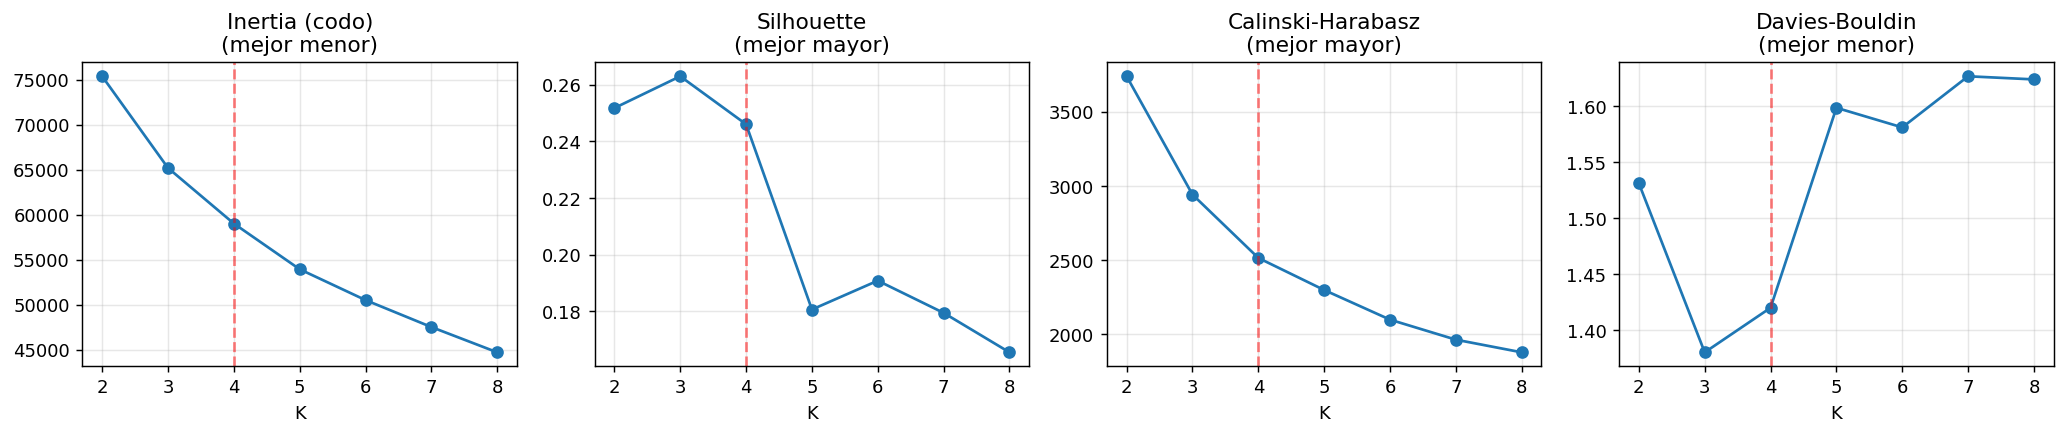
\includegraphics[width=\linewidth]{01_seleccion_k.png}
\caption{Métricas internas para distintos valores de K. La línea roja marca el
valor elegido. K=3 y K=4 muestran métricas muy similares; el desempate se hace
por accionabilidad.}
\label{fig:seleccion_k}
\end{figure}

Las métricas son ligeramente mejores en K=3 (silhouette de 0.26 contra 0.25,
Davies-Bouldin de 1.38 contra 1.42), pero con K=3 el cluster de visitantes
mobile queda diluido dentro del segmento de desktop superficiales. Con K=4 el
segmento mobile emerge como entidad propia, lo cual abre una palanca de
marketing concreta. La diferencia en métricas es marginal y la ganancia
operativa es sustantiva, así que se elige K=4. Este es exactamente el tipo de
decisión donde el criterio cuantitativo se complementa con el criterio de
negocio sin pretender que uno reemplace al otro.

Para confirmar que la elección no es un artefacto del algoritmo, se compararon
tres familias distintas de clustering aplicadas con K=4: KMeans, clustering
aglomerativo con linkage de Ward y Gaussian Mixture Model con covarianza
completa. KMeans y Ward producen soluciones muy parecidas con silhouette de 0.25
y 0.23 respectivamente; el GMM produce una solución diferente con peor
separación geométrica. La concordancia entre KMeans y Ward es una señal fuerte
de que la estructura encontrada no es producto de un algoritmo particular, sino
que refleja patrones reales en los datos. Adicionalmente se exploró HDBSCAN,
cuyo resultado revela algo interesante: con cualquier parámetro razonable
encuentra solamente dos clusters densos, mobile y todo lo demás. Esto se
interpreta como que el cluster mobile es genuinamente denso en el sentido de
densidad espacial, mientras que los otros tres segmentos son particiones
funcionales sobre un continuo de engagement. Esta honestidad analítica vale la
pena explicitarla: los segmentos C0, C1 y C2 son cortes operativos útiles sobre
una nube continua, no agrupaciones naturalmente discretas.

Se eligió KMeans por encima de Ward por una razón operativa: los centroides
permiten asignar visitantes nuevos en producción con una sola operación de
distancia mínima, sin necesidad de recomputar el árbol jerárquico ni almacenar
matrices de covarianza. Este es un punto importante: la elección no solo
favorece la calidad estadística sino también la viabilidad de despliegue.

\section{Validación de robustez y tests estadísticos}

Una segmentación obtenida con un algoritmo no supervisado no tiene etiquetas
verdaderas contra qué comparar. No existe accuracy ni área bajo la curva. La
validación entonces se enfoca en una pregunta distinta: ¿son los clusters
encontrados estables y reproducibles, o son un artefacto de la muestra
específica? Esta pregunta se aborda con tres tipos de pruebas complementarias.

La primera es estabilidad por bootstrap. Se reentrenan treinta modelos KMeans
con muestras del ochenta por ciento del dataset, se asignan los visitantes
completos usando los centroides de cada bootstrap, y se compara cada asignación
con la del modelo base usando el Adjusted Rand Index. El ARI mide acuerdo entre
dos particiones corrigiendo por azar, vale uno cuando son idénticas y cero
cuando son tan parecidas como dos asignaciones aleatorias. El resultado del
ejercicio es un ARI medio de 0.974 con mediana de 0.994. Los clusters reaparecen
casi idénticos con datos distintos.

La segunda prueba es hold-out 80/20. Se entrenan los centroides con el ochenta
por ciento de los datos, se asigna el veinte por ciento restante usando esos
centroides, y se compara el silhouette en el conjunto de entrenamiento contra el
de prueba. Si los clusters fueran un sobreajuste, el silhouette en prueba caería
considerablemente. El resultado es un silhouette de 0.243 tanto en entrenamiento
como en prueba, con una diferencia inferior a una milésima en promedio sobre
diez folds. Los centroides aprendidos en una muestra generalizan a datos no
vistos sin pérdida.

La tercera prueba es robustez al ruido. Se añade perturbación gaussiana con
desviación estándar de 0.1 al dataset escalado y se predice de nuevo con los
centroides originales. El ARI entre las asignaciones originales y las
perturbadas se mantiene en 0.96, lo que significa que solo el cuatro por ciento
de los visitantes cambian de cluster ante perturbaciones pequeñas.

Pasamos luego a la validación estadística formal sobre los clusters obtenidos.
Antes de elegir test, verificamos normalidad con D'Agostino-Pearson dentro de
cada cluster. Ninguna variable es normal en ningún cluster, lo cual lleva a
descartar ANOVA en favor de Kruskal-Wallis. Es importante señalar que con un
tamaño muestral cercano a diez mil, casi cualquier diferencia produce
p-valores prácticamente cero. La interpretación se centra entonces en effect
size, eta-cuadrado para Kruskal-Wallis y V de Cramer para chi-cuadrado, que es
lo que distingue diferencias triviales de diferencias importantes.

La tabla \ref{tab:effect_size} resume el effect size por variable.

\begin{table}[h]
\centering
\caption{Effect size de Kruskal-Wallis por variable numérica.}
\label{tab:effect_size}
\begin{tabular}{lrl}
\toprule
Variable & $\eta^2$ & Magnitud \\
\midrule
hits\_per\_session & 0.645 & grande \\
pageviews\_per\_session & 0.638 & grande \\
n\_sessions & 0.562 & grande \\
totals.pageviews & 0.539 & grande \\
totals.hits & 0.528 & grande \\
weekend\_prop & 0.503 & grande \\
bounce\_prop & 0.257 & grande \\
hour & 0.017 & trivial \\
\bottomrule
\end{tabular}
\end{table}

Siete de ocho variables muestran effect size grande, lo que confirma que los
clusters no son una partición arbitraria sino que capturan diferencias
sustanciales en el comportamiento de los visitantes. La única excepción es
\texttt{hour}, con effect size trivial. La hora del día no separa los clusters,
y esto contradice un supuesto común en marketing digital de que el momento de
la visita es un segmentador relevante.

El post-hoc de Dunn con corrección de Bonferroni permite identificar qué pares
específicos de clusters difieren. El resultado más interesante aparece en
\texttt{hits\_per\_session}: los clusters C0 (Desktop Engaged) y C2 (Weekend
Warriors) no se diferencian estadísticamente en intensidad de engagement por
sesión. Su única diferencia significativa está en \texttt{weekend\_prop}.
Interpretado correctamente, esto significa que C2 no es un tipo de usuario
distinto de C0; es el mismo tipo de usuario activo en un momento de la semana
diferente. Esta clase de matiz no es visible mirando solo la salida del
clustering y solo emerge al aplicar tests formales sobre los resultados.

Para las variables categóricas, el chi-cuadrado con V de Cramer produce el
resultado más relevante para marketing: \texttt{device.deviceCategory} tiene V
de 0.70, una asociación fuerte con la pertenencia a cluster, mientras que
\texttt{channelGrouping} apenas alcanza V de 0.19, asociación débil. La lectura
es clara: el dispositivo es el separador dominante, no el canal de adquisición.
Esto vuelve a contradecir el supuesto frecuente de que el canal debe ser la
dimensión central de cualquier segmentación de marketing.

Finalmente el MANOVA con Wilks' Lambda confirma a nivel multivariado que los
centroides de los cuatro clusters difieren globalmente en el espacio conjunto
de las variables numéricas, con $\Lambda = 0.62$ y p prácticamente cero. Es la
confirmación final de que los grupos son entidades separadas en el espacio
conjunto y no solo en variables individuales.

\section{Resultados: los cuatro segmentos}

La figura \ref{fig:pca} muestra la proyección bidimensional de los visitantes
en el espacio de componentes principales, coloreados por cluster. Las dos
primeras componentes explican aproximadamente la mitad de la varianza, lo
suficiente para que la separación entre grupos sea visualmente clara.

\begin{figure}[h]
\centering
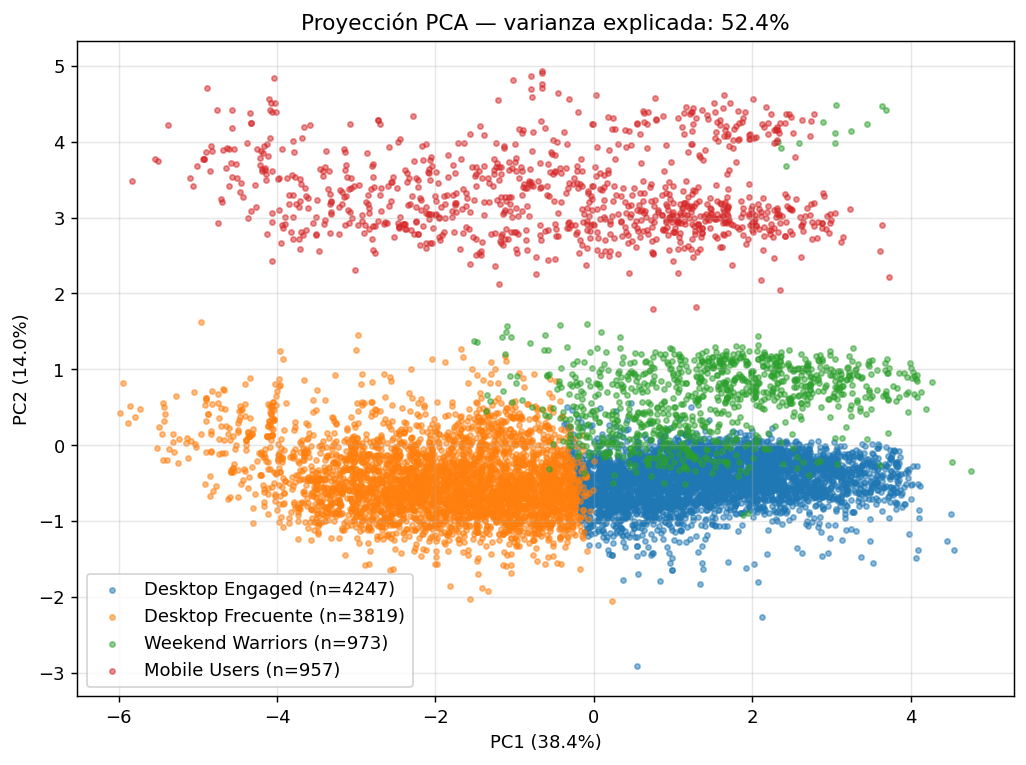
\includegraphics[width=0.85\linewidth]{02_pca_clusters.png}
\caption{Proyección PCA en dos dimensiones de los cuatro segmentos identificados.}
\label{fig:pca}
\end{figure}

\begin{table}[h]
\centering
\caption{Perfil promedio de cada segmento.}
\label{tab:perfiles}
\small
\begin{tabular}{lrrrrrrr}
\toprule
Segmento & n & \% & sesiones & hits/ses & bounce & weekend & mobile \\
\midrule
C0 Desktop Engaged   & 4.247 & 42.5 & 1.65 & 25.21 & 0.01 & 0.01 & 0.00 \\
C1 Desktop Frecuente & 3.819 & 38.2 & 6.36 & 2.14  & 0.15 & 0.10 & 0.00 \\
C2 Weekend Warriors  & 973   & 9.7  & 1.69 & 25.44 & 0.03 & 0.85 & 0.01 \\
C3 Mobile Users      & 957   & 9.6  & 3.28 & 12.69 & 0.17 & 0.25 & 1.00 \\
\bottomrule
\end{tabular}
\end{table}

El segmento Desktop Engaged concentra al 42.5 por ciento de los visitantes y
representa al usuario que visita pocas veces pero con sesiones largas y
profundas. En promedio realizan 1.65 sesiones con veinticinco hits cada una. Su
tasa de rebote es del uno por ciento, prácticamente nula. Llegan
mayoritariamente por canales Direct y Organic Search, lo que sugiere usuarios
con intención de compra ya formada. Este es el segmento que efectivamente
convierte y la prioridad para él no es la atracción sino la conversión: testing
A/B sobre el checkout, mejora de páginas de producto, programas de fidelización
para retener.

El segmento Desktop Frecuente es el más interesante desde el punto de vista
estratégico. Agrupa al 38.2 por ciento de los visitantes y se caracteriza por un
patrón aparentemente contradictorio: vienen muchas veces, en promedio seis
sesiones, pero cada sesión es muy corta, con apenas dos hits. Bounce rate del
quince por ciento. El cincuenta y cinco por ciento llegan por canal Referral,
lo que apunta a lectores de blogs, comparadores o reviews que regresan al sitio
en busca de información puntual. Esta es la audiencia con mayor potencial de
crecimiento. La estrategia adecuada es nurturing con contenido educativo,
emails con valor antes de cualquier promoción, retargeting con guías de producto
en lugar de descuentos.

El segmento Weekend Warriors es pequeño pero homogéneo, con 973 visitantes que
concentran el ochenta y cinco por ciento de sus visitas en sábado y domingo. Su
engagement es equivalente al de Desktop Engaged en términos de hits por sesión
y bounce rate. Como se discutió en la sección de tests estadísticos, el post-hoc
confirma que son indistinguibles de Desktop Engaged en intensidad y solo se
diferencian en el momento de la semana. La interpretación operativa es directa:
son power users con disponibilidad de fin de semana. Las acciones recomendadas
son campañas programadas con dayparting viernes a domingo, mayor inversión en
paid search en esos días y contenido más visual y orientado al ocio.

El segmento Mobile Users agrupa al diez por ciento restante, todos en mobile o
tablet, repartidos casi por mitades entre iOS y Android. Tienen engagement
medio pero un bounce rate del diecisiete por ciento, diecisiete veces el de
Desktop Engaged. La mayor proporción de Paid Search dentro de este cluster
señala algo importante para el negocio: se está pagando para llevar tráfico
mobile a una experiencia que no convierte. Antes de cualquier campaña adicional,
la prioridad debe ser de producto y no de marketing: auditoría de Core Web
Vitals, optimización del peso de imágenes, revisión del flujo de checkout
mobile. Mientras la experiencia no se arregle, incrementar la inversión de
adquisición sobre este segmento es ineficiente.

\begin{figure}[h]
\centering
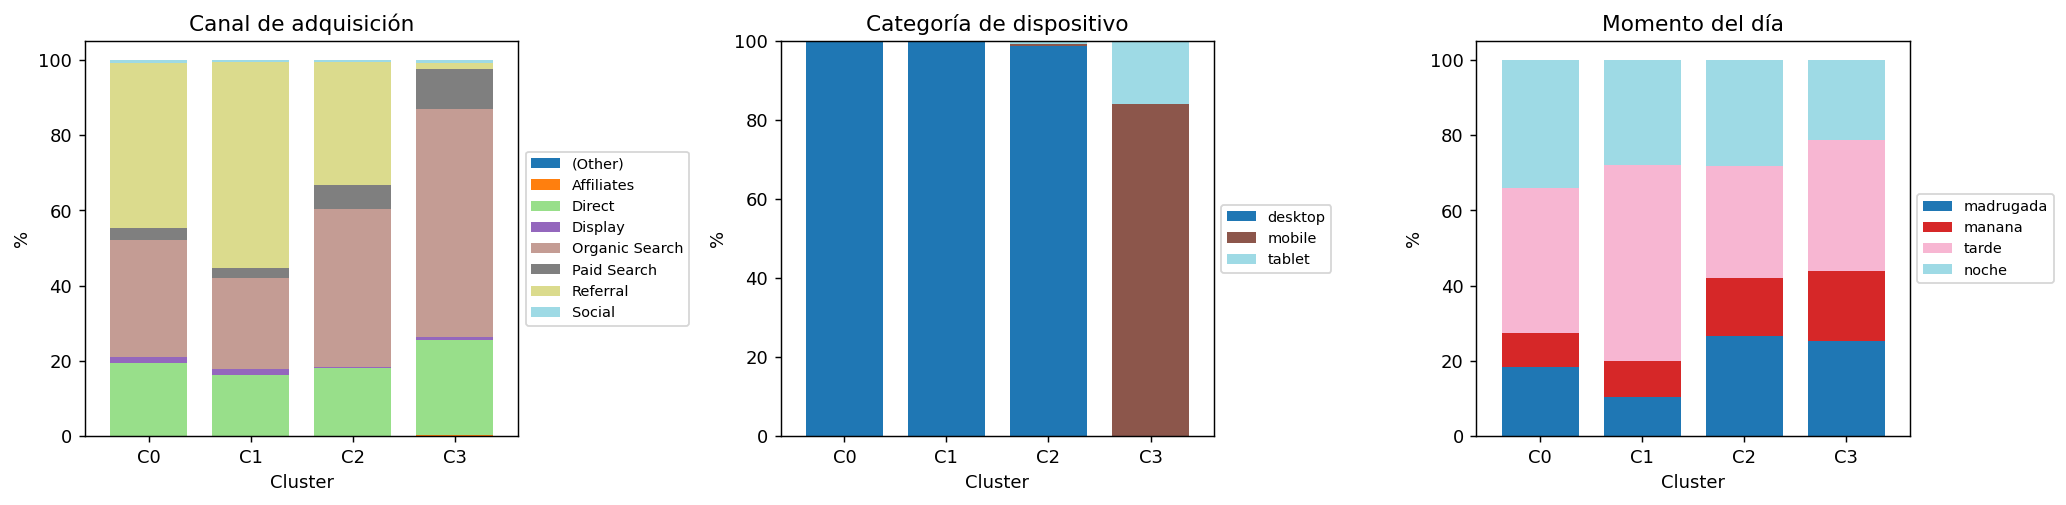
\includegraphics[width=\linewidth]{03_composicion_categorica.png}
\caption{Composición categórica por cluster: canal de adquisición, dispositivo y momento del día.}
\label{fig:categoricas}
\end{figure}

\section{Recomendaciones de marketing}

Las recomendaciones se derivan directamente de los perfiles y de los hallazgos
estadísticos. Para Desktop Engaged el objetivo es maximizar conversión y ticket
medio en una audiencia que ya está convencida, con foco en optimización de la
experiencia de compra y programas de loyalty. Para Desktop Frecuente, donde
está el mayor potencial de crecimiento, la estrategia es nurturing por contenido
con métricas de éxito centradas en aumentar las páginas vistas por sesión y la
profundidad del engagement, no en conversión inmediata. Para Weekend Warriors,
el enfoque es captura en ventana de oportunidad, con campañas programadas y
oferta de tiempo limitado en fines de semana. Para Mobile Users, la recomendación
es atípica: antes de invertir en marketing hay que invertir en producto, porque
el problema observado no es de adquisición sino de experiencia.

Una recomendación transversal que el análisis estadístico justifica es revisar
la asignación de presupuesto entre canales. El dispositivo separa mucho más que
el canal, por lo que campañas pensadas como ``canal Referral'' pueden estar
subóptimamente diseñadas si dentro de ese canal coexisten usuarios desktop con
intent profundo y usuarios mobile con intent superficial.

\section{Limitaciones}

El dataset no contiene variables de conversión, revenue o lifetime value, por lo
que la segmentación captura comportamiento de engagement pero no valor de
negocio. Una iteración natural sería complementar este trabajo con una
segmentación por valor (modelo RFM o LTV) que requiere datos transaccionales.
También sería valioso validar cualitativamente los segmentos con el equipo de
marketing, revisando una muestra de treinta a cincuenta visitantes por cluster
y verificando que los perfiles coinciden con lo que observan en el día a día.
Por último, la composición del dataset apunta fuertemente a tratarse de la
muestra del Google Merchandise Store, con su sesgo característico hacia
Chrome y Macintosh; los segmentos mobile en particular están construidos sobre
una minoría del diez por ciento del dataset y conviene tomar sus conclusiones
con cautela en consecuencia.

\section{Conclusiones}

El trabajo entrega una segmentación accionable en cuatro grupos diferenciados,
con cada grupo respaldado por effect sizes grandes en variables clave y con la
estabilidad confirmada bajo bootstrap y hold-out. Más allá del resultado, el
ejercicio aporta dos hallazgos que un análisis menos riguroso podría pasar por
alto. El primero, que dos de los cuatro segmentos (Desktop Engaged y Weekend
Warriors) son funcionalmente equivalentes en su intensidad de engagement y solo
se diferencian en el momento de la semana en que actúan; reconocerlo permite
diseñar estrategias más eficientes que tratan al mismo usuario con el contenido
adecuado para cada ventana de tiempo. El segundo, que el dispositivo es el
separador dominante por encima del canal de adquisición, lo cual reorienta las
prioridades de inversión: mejorar la experiencia mobile rinde más que aumentar
el presupuesto de adquisición sobre una experiencia que no convierte.

\end{document}
